
\chapter{Testowanie}
\section{Frontend}
Testy w części frondendowej aplikacji wykonywane są przy pomocy platformy programistycznej Jest. W projekcie można wyróżnić podział na dwa typy testów. Pierwszym typem są testy spójności magazynu Vuex. Przykładowym testem tego typu jest test przypisanie tokenu JWT~(zob.~listing~\ref{lst:vuextest}). Celem testu jest sprawdzenie, czy funkcje odpowiadające za zapisywanie i odczytywanie danych zostały poprawnie zdefiniowane.
\begin{lstlisting}[caption=Test spójności magazynu Vuex,label={lst:vuextest}] 
describe('mutations', () => {
  test('setToken', () => {
    const token = "exampletoken"
    const state = {
      token: ""
    }
    store.commit('SET_TOKEN', { token })
    expect(store.getters.getToken.token).toBe(token)
  })
\end{lstlisting}

Drugim typem testów są testy interfejsu użytkownika. Przykładem takiego testu jest test przycisku, który odpowiada za zwiększanie liczby prowadzonych przez nauczyciela przedmiotów~(zob.~listing~\ref{lst:uitest}). Celem testu jest sprawdzenie, czy akcja wykonana przez użytkownika, w tym przypadku symulowana, skutkuje odpowiednią zmianą zmiennych w kodzie aplikacji. 
\begin{lstlisting}[caption=Test interfejsu użytkownika,label={lst:uitest}] 
describe('userInput', () => {
  test('addSubject', async () => {
    const wrapper = mount(Step2)
    const button = wrapper.find('addSubjectButton')

    expect(subjectNumber).toBe(0)
    await button.trigger('click')
    expect(subjectNumber).toBe(1)
})})
\end{lstlisting}
\section{Backend}
\subsection{Testowanie manualne}

Część backendowa, testowana była w dużym stopniu manualnie. Głównym narzędziem była aplikacja Postman. Przykładowe zapytanie wraz z odpowiedzią pokazano na rysunku ~\ref{rys:postman}.

\begin{figure}[H]
	\centering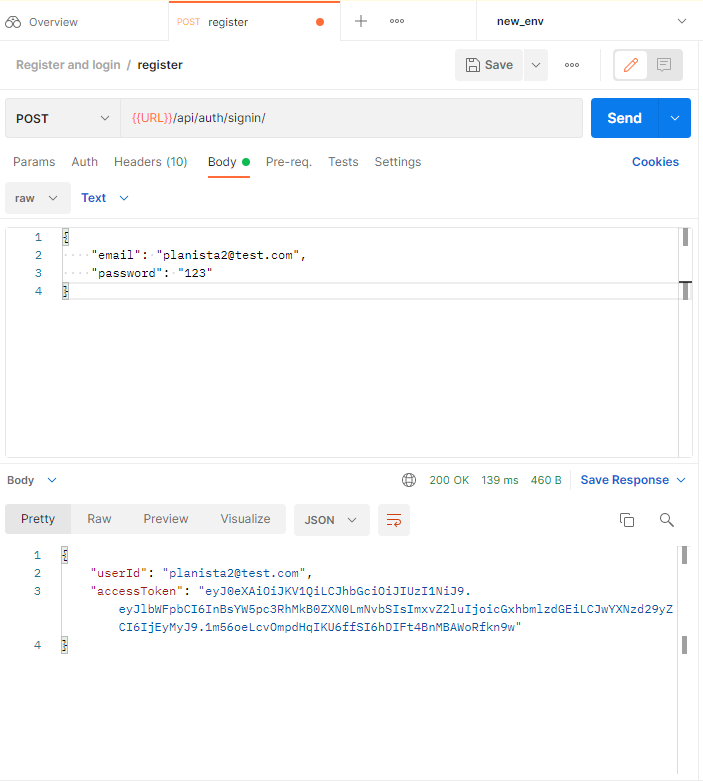
\includegraphics[width=\textwidth]{figures/postman1}
	\caption{Przykładowe zapytanie oraz odpowiedź w Postman}\label{rys:postman}
\end{figure}

Na zaawansowanych etapach implementacji, testy wykonywane były również z pomocą aplikacji frontendowej, dzięki czemu można była na bieżąco weryfikować integrację.

\subsection{Testy automatyczne}
Testami automatycznymi objęte zostały widoki oraz adresy URL. Do testowania widoków, wykorzystywane są testy integracyjne, natomiast do adresów testy jednostkowe. W obu przypadkach wykorzystywane są gotowe rozwiązania zaimplementowane w Django. Testy jednostkowe, sprawdzające poprawność implementacji adresów internetowych, sprawdzają czy podczas wysłania zapytania na dany adres, wywoływana jest opowiednia funkcja. Przykład implementacji takiego testu na listingu ~\ref{lst:TestJednostkowyBackend}.

\begin{lstlisting}[language=Python, caption=Implementacja przykładowego testu jednostkowego, label={lst:TestJednostkowyBackend}]
	class TestUrls(SimpleTestCase):
	
		def test_add_user(self):
			url = reverse('user')
			self.assertEquals(resolve(url).func, add_user)
\end{lstlisting}

Natomiast testy integracyjne, odpowiadające za widoki, mają za zadanie sprawdzić czy widok zwrócił odpowiednią odpowiedź HTPP. Przykład takiego testu na listingu ~\ref{lst:TestIntegracyjnyBackend}.

\begin{lstlisting}[language=Python, caption=Implementacja przykładowego testu integracyjnego, label={lst:TestIntegracyjnyBackend}]
	class TestViews(TestCase):
	
		def test_add_user_POST(self):
	
			email = 'test1@test2@.com'
			client = Client()
			url = reverse('user')
			
			Planners.objects.create(
			planneremail = email,
			login = 'test',
			password = 'test'
			)
			
			response = client.post(url, {
				'Sukces': 'Pomyslnie dodano uzytkownika'
			})
			
			self.assertEquals(response.status_code, 200)
\end{lstlisting}


\section{Algorytm}
	\subsection{Testy manualne}
	Testy manualne algorytmu przeprowadzane były przy pomocy przykładowych danych pierwotnie przygotowanych przez grupę inżynierską oraz ostatecznie uzyskanych z przykładowej istniejącej szkoły średniej. Dzięki wykorzystaniu danych z prawdziwej szkoły powstałą możliwość porównania planów generowanych przez algorytm z planem stworzonym przez wyszkolonego planistę w szkole średniej.	Dzięki temu możliwe było zwrócenie uwagi na niedoskonałości planu wygenerowanego względem tego stworzonego przez planistę oraz wyeliminowanie ich. Dzięki takim testom manualnym plany generowane przez algorytm udało się doprowadzić do stanu co najmniej bliskiego w stosunku do planu stworzonego przez wyszkolonego planistę.
	
	\subsection{Testy automatyczne}	
	Automatyczne testy jednostkowe algorytmu odbywają się przy pomocy biblioteki \textit{pytest}. Dzięki tej bibliotece testy napisane w języku Python można wywóływać przy pomocy jednej komendy. Przykładowym testem jednostkowym jest sprawdzenie czy dane uzyskane z backendu zostały prawidłowo przetworzone przez algorytm w celu ułatwienia wykonywania na nich różnych operacji. Poniższy test sprawdza, czy ilość danych przygotowanych dla algorytmu zgadza się z ilością otrzymanych danych (zob.~listing~\ref{lst:test_data}).
	\begin{lstlisting}[language=Python, caption=Implementacja przykładowego testu jednostkowego sprawdzającego spójność danych, label={lst:test_data}]
	def test_data_structures(groups_data=GROUP_OLD, teachers_data=TEACHERS_OLD, classrooms_data=CLASSES_OLD):
    school = School(groups_data, teachers_data, classrooms_data)
    assert len(school.groups) == len(groups_data), "Groups copied incorrectly to dict of class Group"
    assert len(school.classrooms) == len(classrooms_data), "Classrooms copied incorrectly to dict of class Classroom"
    assert len(school.teachers) == len(teachers_data), "Teachers copied incorrectly to dict of class Teacher"
\end{lstlisting}
	
	Kolejnym przykładem automatycznego testu jednostkowego jest sprawdzenie samego procesu ewolucji. Ocena gotowego najlepszego planu z pierwszego pokolenia jest zapisywana. Następnie przeprowadzony zostaje proces ewolucji. Ocena najlepszego planu uzyskanego z ostatniego pokolenia jest zapisywana. Podczas testu sprawdzane jest czy ocena uzyskana przez plan po procesie ewolucji jest lepsza, niż planu przed rozpoczęciem ewolucji (zob.~listing~\ref{lst:test_evolution}).
	
	\begin{lstlisting}[language=Python, caption=Implementacja przykładowego testu jednostkowego sprawdzającego proces ewolucji, label={lst:test_evolution}]
	def test_evolution(groups_data=GROUP_OLD, teachers_data=TEACHERS_OLD, classrooms_data=CLASSES_OLD):
    population_size = 10
    num_of_generations = 100
    num_of_mutations = 20

    population = Population(groups_data=groups_data, teachers_data=teachers_data, classrooms_data=classrooms_data)
    population.new_population(number_of_instances=population_size)
    before_evolution = population.get_best_specimen().evaluation
    population.evolute(num_of_generations, num_of_mutations)
    after_evolution = population.get_best_specimen().evaluation

    assert before_evolution < after_evolution, "Before evaluation is not smaller than after evaluation"
    print("Evaluation before evolution is smaller than after evolution")
\end{lstlisting}


	\subsection{Testy jakościowe i wydajnościowe}
	Wykonano testy jakościowe oraz wydajnościowe dla przykładowego zestawu danych. Dane pochodziły z prawdziwej szkoły średniej dzięki czemu możliwe było odniesienie wyników do warunków rzeczywistych. Po przetworzeniu danych otrzymane została lista krotek o długości 602. Przeprowadzony zostały po 4 testy dla różnych ustawień algorytmu. 
\begin{itemize}
	\item Pierwszy zestaw testów został przeprowadzony dla ustawień algorytmu w postaci: rozmiar populacji = 10, liczba pokoleń = 5000, liczba mutacji = 3\% liczby krotek w liście (zaokrąglone w dół). Zauważyć można bardzo niską powtarzalność otrzymanych wyników (zob.~rysunek~\ref{rys:graph_3}). Wynika to z dość dużej ilości wprowadzanych losowych zmian w jednym czasie. Przez taki zabieg plan zajęć mocno zatraca element ewolucji. 
	\newpage
	\item Drugi zestaw testów przeprowadzony został dla następujących ustawień algorytmu: rozmiar populacji = 10, liczba pokoleń = 5000, liczba mutacji = 2\% liczby krotek w liście (zaokrąglone w dół). Zauważyć można delikatny wzrost powtarzalności wyników idący w parze ze wzrostem otrzymanej finalnej oceny planu zajęć (zob.~rysunek~\ref{rys:graph_2}). 
	\item Trzeci zestaw testów wykonany został dla ustawień algorytmu w postaci: rozmiar populacji = 10, liczba pokoleń = 5000, liczba mutacji = 1\% liczby krotek w liście (zaokrąglone w dół). Dla tych ustawień zauważyć można delikatnie zwiększoną powtarzalność uzyskiwanych wyników wraz z minimalnym wzrostem uzyskanej oceny końcowej względem liczby mutacji wynoszącej 2\% (zob.~rysunek~\ref{rys:graph_1}). 
	\item Czwarty zestaw testów został wykonany dla następujących parametrów przyjętych przez algorytm:  rozmiar populacji = 10, liczba pokoleń = 5000, liczba mutacji = 0.5\% liczby krotek w liście (zaokrąglone w dół). Dla takiego zestawu ustawień można zauważyć zarówno ogromny wzrost powtarzalności uzyskiwanych wyników jak i bardzo wysoki wynik końcowy ocenianych planów zajęć (zob.~rysunek~\ref{rys:graph_0_5}). 
\end{itemize}
	
	Niestety liczba mutacji w postaci 0.5\% liczby krotek dla tego zestawu danych mocno zbliżyła się do minimalnej wartości jaką może przyjąć algorytm dla tego parametru (2) dlatego w tym miejscu testowanie z tak przyjętymi parametrami zostało zakończone. Każdy pojedynczy test z przedstawionych zestawów został wykonany zarówno na komputerze osobistym o specyfikacji (Intel Core i7 4790k, 16GB RAM DDR3-1866MHz) jak i instancji AWS EC2 t2.micro (1 core, 1GB RAM). Dla obu platform czas przebiegu testu (wygenerowania planu o otrzymanej ocenie końcowej) był mocno powtarzalny jednak znacznie się różniący pomiędzy platformami. Komputerowi osobistemu wykonanie jednego testu zajęło ok. 4 minut. Instancji t2.micro wykonanie jednego testu zajęło ok. 30 minut. 	
\begin{figure}[H]
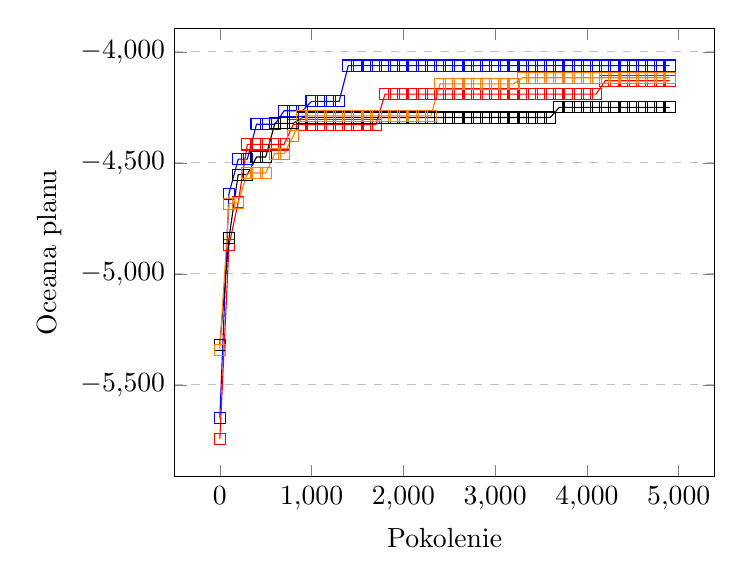
\begin{tikzpicture}
\begin{axis}[
    xlabel={Pokolenie},
    ylabel={Oceana planu},
    ymajorgrids=true,
    grid style=dashed,
]

\addplot[
    color=blue,
    mark=square,
    ]
    coordinates {
(0, -5649.799999999999)(100, -4638.799999999999)(200, -4483.5999999999985)(300, -4483.5999999999985)(400, -4326.4)(500, -4326.4)(600, -4326.4)(700, -4265.599999999999)(800, -4265.599999999999)(900, -4265.599999999999)(1000, -4222.999999999999)(1100, -4222.999999999999)(1200, -4222.999999999999)(1300, -4222.999999999999)(1400, -4061.9999999999995)(1500, -4061.9999999999995)(1600, -4061.9999999999995)(1700, -4061.9999999999995)(1800, -4061.9999999999995)(1900, -4061.9999999999995)(2000, -4061.9999999999995)(2100, -4061.9999999999995)(2200, -4061.9999999999995)(2300, -4061.9999999999995)(2400, -4061.9999999999995)(2500, -4061.9999999999995)(2600, -4061.9999999999995)(2700, -4061.9999999999995)(2800, -4061.9999999999995)(2900, -4061.9999999999995)(3000, -4061.9999999999995)(3100, -4061.9999999999995)(3200, -4061.9999999999995)(3300, -4061.9999999999995)(3400, -4061.9999999999995)(3500, -4061.9999999999995)(3600, -4061.9999999999995)(3700, -4061.9999999999995)(3800, -4061.9999999999995)(3900, -4061.9999999999995)(4000, -4061.9999999999995)(4100, -4061.9999999999995)(4200, -4061.9999999999995)(4300, -4061.9999999999995)(4400, -4061.9999999999995)(4500, -4061.9999999999995)(4600, -4061.9999999999995)(4700, -4061.9999999999995)(4800, -4061.9999999999995)(4900, -4061.9999999999995)
    };
    
\addplot[
    color=red,
    mark=square,
    ]
    coordinates {
(0, -5745.000000000001)(100, -4872.0)(200, -4678.8)(300, -4417.399999999999)(400, -4417.399999999999)(500, -4417.399999999999)(600, -4417.399999999999)(700, -4417.399999999999)(800, -4328.2)(900, -4328.2)(1000, -4328.2)(1100, -4328.2)(1200, -4328.2)(1300, -4328.2)(1400, -4328.2)(1500, -4328.2)(1600, -4328.2)(1700, -4328.2)(1800, -4190.399999999998)(1900, -4190.399999999998)(2000, -4190.399999999998)(2100, -4190.399999999998)(2200, -4190.399999999998)(2300, -4190.399999999998)(2400, -4190.399999999998)(2500, -4190.399999999998)(2600, -4190.399999999998)(2700, -4190.399999999998)(2800, -4190.399999999998)(2900, -4190.399999999998)(3000, -4190.399999999998)(3100, -4190.399999999998)(3200, -4190.399999999998)(3300, -4190.399999999998)(3400, -4190.399999999998)(3500, -4190.399999999998)(3600, -4190.399999999998)(3700, -4190.399999999998)(3800, -4190.399999999998)(3900, -4190.399999999998)(4000, -4190.399999999998)(4100, -4190.399999999998)(4200, -4130.4)(4300, -4130.4)(4400, -4130.4)(4500, -4130.4)(4600, -4130.4)(4700, -4130.4)(4800, -4130.4)(4900, -4130.4)
    };
    
\addplot[
    color=black,
    mark=square,
    ]
    coordinates {
(0, -5320.5999999999985)(100, -4839.4)(200, -4553.4)(300, -4553.4)(400, -4473.999999999999)(500, -4473.999999999999)(600, -4322.4)(700, -4322.4)(800, -4322.4)(900, -4295.999999999999)(1000, -4295.999999999999)(1100, -4295.999999999999)(1200, -4295.999999999999)(1300, -4295.999999999999)(1400, -4295.999999999999)(1500, -4295.999999999999)(1600, -4295.999999999999)(1700, -4295.999999999999)(1800, -4295.999999999999)(1900, -4295.999999999999)(2000, -4295.999999999999)(2100, -4295.999999999999)(2200, -4295.999999999999)(2300, -4295.999999999999)(2400, -4295.999999999999)(2500, -4295.999999999999)(2600, -4295.999999999999)(2700, -4295.999999999999)(2800, -4295.999999999999)(2900, -4295.999999999999)(3000, -4295.999999999999)(3100, -4295.999999999999)(3200, -4295.999999999999)(3300, -4295.999999999999)(3400, -4295.999999999999)(3500, -4295.999999999999)(3600, -4295.999999999999)(3700, -4249.999999999999)(3800, -4249.999999999999)(3900, -4249.999999999999)(4000, -4249.999999999999)(4100, -4249.999999999999)(4200, -4249.999999999999)(4300, -4249.999999999999)(4400, -4249.999999999999)(4500, -4249.999999999999)(4600, -4249.999999999999)(4700, -4249.999999999999)(4800, -4249.999999999999)(4900, -4249.999999999999)
    };
    
\addplot[
    color=orange,
    mark=square,
    ]
    coordinates {
(0, -5342.200000000001)(100, -4684.400000000001)(200, -4679.999999999999)(300, -4545.799999999999)(400, -4545.799999999999)(500, -4545.799999999999)(600, -4458.799999999999)(700, -4458.799999999999)(800, -4379.800000000001)(900, -4288.800000000001)(1000, -4288.800000000001)(1100, -4288.800000000001)(1200, -4288.800000000001)(1300, -4288.800000000001)(1400, -4288.800000000001)(1500, -4288.800000000001)(1600, -4288.800000000001)(1700, -4288.800000000001)(1800, -4288.800000000001)(1900, -4288.800000000001)(2000, -4288.800000000001)(2100, -4288.800000000001)(2200, -4288.800000000001)(2300, -4288.800000000001)(2400, -4144.4)(2500, -4144.4)(2600, -4144.4)(2700, -4144.4)(2800, -4144.4)(2900, -4144.4)(3000, -4144.4)(3100, -4144.4)(3200, -4144.4)(3300, -4116.999999999999)(3400, -4116.999999999999)(3500, -4116.999999999999)(3600, -4116.999999999999)(3700, -4116.999999999999)(3800, -4116.999999999999)(3900, -4116.999999999999)(4000, -4116.999999999999)(4100, -4116.999999999999)(4200, -4116.999999999999)(4300, -4116.999999999999)(4400, -4116.999999999999)(4500, -4116.999999999999)(4600, -4116.999999999999)(4700, -4116.999999999999)(4800, -4116.999999999999)(4900, -4116.999999999999)
    };

\end{axis}
\end{tikzpicture}
\caption{Zmiana oceny planu podczas ewolucji badana co 100 pokoleń. \newline
Rozmiar populacji = 10, Liczba pokoleń = 5000, Liczba mutacji = 3\% krotek \newline
(więcej=lepiej)}\label{rys:graph_3}
\end{figure}

\begin{figure}[H]
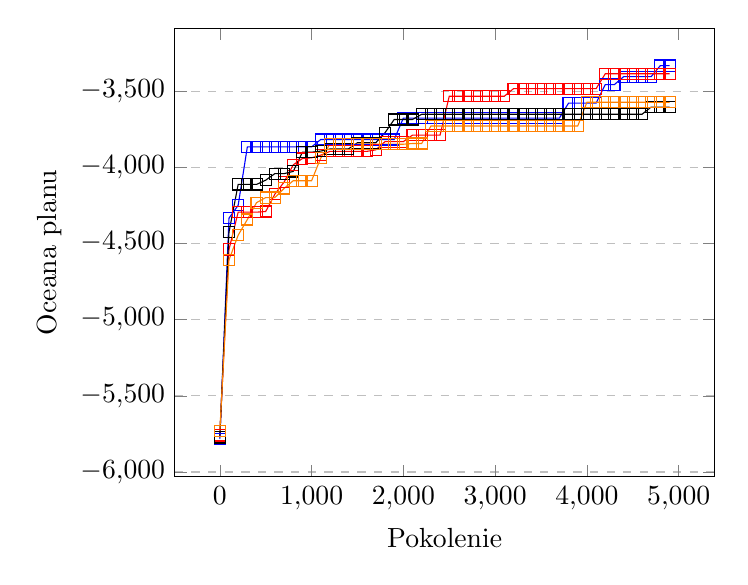
\begin{tikzpicture}
\begin{axis}[
    xlabel={Pokolenie},
    ylabel={Oceana planu},
    ymajorgrids=true,
    grid style=dashed,
]

\addplot[
    color=blue,
    mark=square,
    ]
    coordinates {
(0, -5784.4000000000015)(100, -4332.800000000001)(200, -4248.2)(300, -3864.7999999999997)(400, -3864.7999999999997)(500, -3864.7999999999997)(600, -3864.7999999999997)(700, -3864.7999999999997)(800, -3864.7999999999997)(900, -3864.7999999999997)(1000, -3864.7999999999997)(1100, -3816.0)(1200, -3816.0)(1300, -3816.0)(1400, -3816.0)(1500, -3816.0)(1600, -3816.0)(1700, -3816.0)(1800, -3816.0)(1900, -3816.0)(2000, -3675.5999999999995)(2100, -3675.5999999999995)(2200, -3675.5999999999995)(2300, -3675.5999999999995)(2400, -3675.5999999999995)(2500, -3675.5999999999995)(2600, -3675.5999999999995)(2700, -3675.5999999999995)(2800, -3675.5999999999995)(2900, -3675.5999999999995)(3000, -3675.5999999999995)(3100, -3675.5999999999995)(3200, -3675.5999999999995)(3300, -3675.5999999999995)(3400, -3675.5999999999995)(3500, -3675.5999999999995)(3600, -3675.5999999999995)(3700, -3675.5999999999995)(3800, -3576.999999999999)(3900, -3576.999999999999)(4000, -3576.999999999999)(4100, -3576.999999999999)(4200, -3455.1999999999994)(4300, -3455.1999999999994)(4400, -3403.4)(4500, -3403.4)(4600, -3403.4)(4700, -3403.4)(4800, -3330.599999999999)(4900, -3330.599999999999)
    };
    
    \addplot[
    color=red,
    mark=square,
    ]
    coordinates {
(0, -5759.8)(100, -4538.200000000001)(200, -4293.4)(300, -4293.4)(400, -4293.4)(500, -4289.0)(600, -4175.000000000001)(700, -4096.0)(800, -3982.4000000000005)(900, -3941.0000000000005)(1000, -3936.2000000000003)(1100, -3919.000000000001)(1200, -3894.2000000000003)(1300, -3894.2000000000003)(1400, -3894.2000000000003)(1500, -3894.2000000000003)(1600, -3894.2000000000003)(1700, -3884.2000000000003)(1800, -3830.0000000000005)(1900, -3830.0000000000005)(2000, -3830.0000000000005)(2100, -3787.0)(2200, -3787.0)(2300, -3787.0)(2400, -3787.0)(2500, -3531.7999999999997)(2600, -3531.7999999999997)(2700, -3531.7999999999997)(2800, -3531.7999999999997)(2900, -3531.7999999999997)(3000, -3531.7999999999997)(3100, -3531.7999999999997)(3200, -3482.2)(3300, -3482.2)(3400, -3482.2)(3500, -3482.2)(3600, -3482.2)(3700, -3482.2)(3800, -3482.2)(3900, -3482.2)(4000, -3482.2)(4100, -3482.2)(4200, -3384.3999999999996)(4300, -3384.3999999999996)(4400, -3384.3999999999996)(4500, -3384.3999999999996)(4600, -3384.3999999999996)(4700, -3384.3999999999996)(4800, -3384.3999999999996)(4900, -3384.3999999999996)
    };
    
        \addplot[
    color=black,
    mark=square,
    ]
    coordinates {
(0, -5772.799999999999)(100, -4424.8)(200, -4111.2)(300, -4111.2)(400, -4111.2)(500, -4083.2)(600, -4040.2000000000003)(700, -4040.2000000000003)(800, -4025.8)(900, -3899.600000000001)(1000, -3899.600000000001)(1100, -3892.2)(1200, -3878.6)(1300, -3878.6)(1400, -3878.6)(1500, -3837.1999999999994)(1600, -3837.1999999999994)(1700, -3837.1999999999994)(1800, -3771.7999999999997)(1900, -3684.6)(2000, -3684.6)(2100, -3684.6)(2200, -3650.3999999999996)(2300, -3650.3999999999996)(2400, -3650.3999999999996)(2500, -3650.3999999999996)(2600, -3650.3999999999996)(2700, -3650.3999999999996)(2800, -3650.3999999999996)(2900, -3650.3999999999996)(3000, -3650.3999999999996)(3100, -3650.3999999999996)(3200, -3650.3999999999996)(3300, -3650.3999999999996)(3400, -3650.3999999999996)(3500, -3650.3999999999996)(3600, -3650.3999999999996)(3700, -3650.3999999999996)(3800, -3650.3999999999996)(3900, -3650.3999999999996)(4000, -3650.3999999999996)(4100, -3650.3999999999996)(4200, -3650.3999999999996)(4300, -3650.3999999999996)(4400, -3650.3999999999996)(4500, -3650.3999999999996)(4600, -3650.3999999999996)(4700, -3602.9999999999995)(4800, -3602.9999999999995)(4900, -3602.9999999999995)
    };
    
            \addplot[
    color=orange,
    mark=square,
    ]
    coordinates {
(0, -5731.999999999999)(100, -4607.399999999999)(200, -4444.6)(300, -4341.6)(400, -4231.0)(500, -4197.6)(600, -4197.6)(700, -4137.599999999999)(800, -4086.7999999999993)(900, -4086.7999999999993)(1000, -4086.7999999999993)(1100, -3937.7999999999997)(1200, -3846.9999999999995)(1300, -3846.9999999999995)(1400, -3846.9999999999995)(1500, -3846.9999999999995)(1600, -3846.9999999999995)(1700, -3846.9999999999995)(1800, -3846.9999999999995)(1900, -3846.9999999999995)(2000, -3846.9999999999995)(2100, -3842.3999999999996)(2200, -3842.3999999999996)(2300, -3727.599999999999)(2400, -3727.599999999999)(2500, -3727.599999999999)(2600, -3727.599999999999)(2700, -3727.599999999999)(2800, -3727.599999999999)(2900, -3727.599999999999)(3000, -3727.599999999999)(3100, -3727.599999999999)(3200, -3727.599999999999)(3300, -3727.599999999999)(3400, -3727.599999999999)(3500, -3727.599999999999)(3600, -3727.599999999999)(3700, -3727.599999999999)(3800, -3727.599999999999)(3900, -3727.599999999999)(4000, -3571.1999999999994)(4100, -3571.1999999999994)(4200, -3571.1999999999994)(4300, -3571.1999999999994)(4400, -3571.1999999999994)(4500, -3571.1999999999994)(4600, -3571.1999999999994)(4700, -3571.1999999999994)(4800, -3571.1999999999994)(4900, -3571.1999999999994)
    };

\end{axis}
\end{tikzpicture}
\caption{Zmiana oceny planu podczas ewolucji badana co 100 pokoleń. \newline
Rozmiar populacji = 10, Liczba pokoleń = 5000, Liczba mutacji = 2\% krotek \newline
(więcej=lepiej)}\label{rys:graph_2}
\end{figure}

\begin{figure}[H]
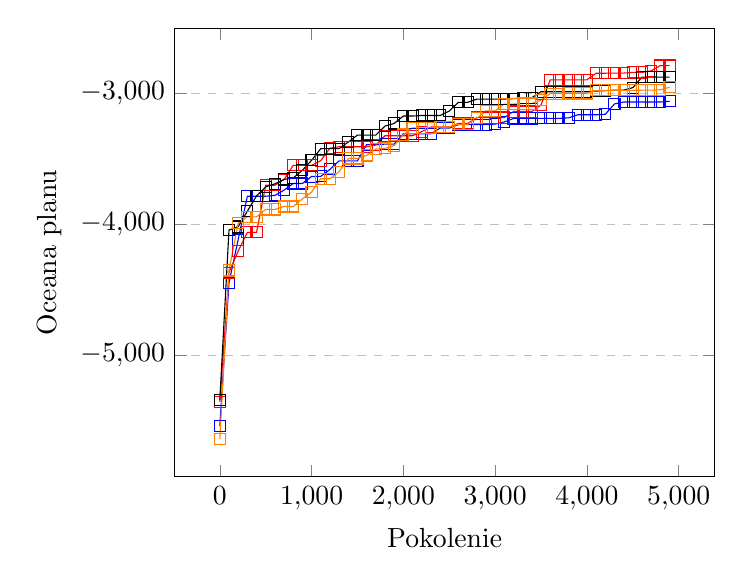
\begin{tikzpicture}
\begin{axis}[
    xlabel={Pokolenie},
    ylabel={Oceana planu},
    ymajorgrids=true,
    grid style=dashed,
]

\addplot[
    color=blue,
    mark=square,
    ]
    coordinates {
(0, -5540.8)(100, -4448.199999999999)(200, -4117.199999999999)(300, -3786.199999999999)(400, -3786.199999999999)(500, -3786.199999999999)(600, -3780.199999999999)(700, -3739.599999999999)(800, -3689.199999999999)(900, -3689.199999999999)(1000, -3635.999999999999)(1100, -3634.3999999999996)(1200, -3581.399999999999)(1300, -3515.999999999999)(1400, -3515.999999999999)(1500, -3515.999999999999)(1600, -3392.1999999999994)(1700, -3392.1999999999994)(1800, -3388.7999999999993)(1900, -3388.7999999999993)(2000, -3309.5999999999995)(2100, -3309.5999999999995)(2200, -3309.5999999999995)(2300, -3309.5999999999995)(2400, -3266.999999999999)(2500, -3266.999999999999)(2600, -3239.999999999999)(2700, -3239.999999999999)(2800, -3239.999999999999)(2900, -3239.999999999999)(3000, -3235.599999999999)(3100, -3219.5999999999995)(3200, -3192.5999999999995)(3300, -3192.5999999999995)(3400, -3192.5999999999995)(3500, -3191.999999999999)(3600, -3191.999999999999)(3700, -3191.999999999999)(3800, -3187.999999999999)(3900, -3164.7999999999997)(4000, -3164.7999999999997)(4100, -3164.7999999999997)(4200, -3160.7999999999997)(4300, -3082.0)(4400, -3067.4)(4500, -3067.4)(4600, -3067.4)(4700, -3067.4)(4800, -3067.4)(4900, -3061.2)
    };
    
\addplot[
    color=red,
    mark=square,
    ]
    coordinates {
(0, -5358.2)(100, -4369.4)(200, -4205.199999999999)(300, -4062.4)(400, -4062.4)(500, -3702.7999999999997)(600, -3702.7999999999997)(700, -3658.7999999999997)(800, -3550.4)(900, -3550.4)(1000, -3550.4)(1100, -3515.1999999999994)(1200, -3419.1999999999994)(1300, -3408.3999999999996)(1400, -3408.3999999999996)(1500, -3408.3999999999996)(1600, -3408.3999999999996)(1700, -3395.799999999999)(1800, -3324.3999999999996)(1900, -3324.3999999999996)(2000, -3324.3999999999996)(2100, -3324.3999999999996)(2200, -3293.3999999999996)(2300, -3257.7999999999993)(2400, -3257.7999999999993)(2500, -3257.7999999999993)(2600, -3230.9999999999995)(2700, -3230.9999999999995)(2800, -3185.9999999999995)(2900, -3185.9999999999995)(3000, -3185.9999999999995)(3100, -3185.9999999999995)(3200, -3139.7999999999997)(3300, -3139.7999999999997)(3400, -3139.7999999999997)(3500, -3090.0)(3600, -2898.0000000000005)(3700, -2898.0000000000005)(3800, -2898.0000000000005)(3900, -2898.0000000000005)(4000, -2898.0000000000005)(4100, -2847.4)(4200, -2847.4)(4300, -2846.4)(4400, -2846.4)(4500, -2841.4)(4600, -2841.4)(4700, -2828.7999999999997)(4800, -2789.2000000000003)(4900, -2789.2000000000003)
    };
    
\addplot[
    color=black,
    mark=square,
    ]
    coordinates {
(0, -5341.799999999998)(100, -4044.9999999999995)(200, -4017.999999999999)(300, -3901.0)(400, -3783.7999999999993)(500, -3715.1999999999994)(600, -3691.7999999999997)(700, -3657.999999999999)(800, -3646.5999999999995)(900, -3588.199999999999)(1000, -3512.1999999999994)(1100, -3423.1999999999994)(1200, -3423.1999999999994)(1300, -3423.1999999999994)(1400, -3372.7999999999997)(1500, -3319.5999999999995)(1600, -3319.5999999999995)(1700, -3319.5999999999995)(1800, -3250.5999999999995)(1900, -3230.5999999999995)(2000, -3173.9999999999995)(2100, -3173.9999999999995)(2200, -3170.0)(2300, -3170.0)(2400, -3170.0)(2500, -3136.2)(2600, -3069.6)(2700, -3069.6)(2800, -3045.6)(2900, -3045.6)(3000, -3045.6)(3100, -3044.4)(3200, -3041.5999999999995)(3300, -3033.9999999999995)(3400, -3033.9999999999995)(3500, -2988.9999999999995)(3600, -2988.9999999999995)(3700, -2988.9999999999995)(3800, -2988.9999999999995)(3900, -2988.9999999999995)(4000, -2988.9999999999995)(4100, -2983.6)(4200, -2980.6)(4300, -2976.6)(4400, -2976.6)(4500, -2957.6)(4600, -2876.7999999999997)(4700, -2876.7999999999997)(4800, -2876.7999999999997)(4900, -2876.7999999999997)
    };
    
\addplot[
    color=orange,
    mark=square,
    ]
    coordinates {
(0, -5640.599999999999)(100, -4352.799999999999)(200, -3992.799999999999)(300, -3943.799999999999)(400, -3943.799999999999)(500, -3886.9999999999986)(600, -3886.9999999999986)(700, -3864.5999999999995)(800, -3864.5999999999995)(900, -3806.399999999999)(1000, -3754.799999999999)(1100, -3652.7999999999997)(1200, -3652.7999999999997)(1300, -3599.0)(1400, -3498.2)(1500, -3498.2)(1600, -3475.2)(1700, -3425.7999999999997)(1800, -3420.9999999999995)(1900, -3399.9999999999995)(2000, -3315.7999999999997)(2100, -3264.7999999999997)(2200, -3264.7999999999997)(2300, -3264.7999999999997)(2400, -3257.7999999999997)(2500, -3257.7999999999997)(2600, -3237.7999999999997)(2700, -3237.7999999999997)(2800, -3191.2)(2900, -3134.9999999999995)(3000, -3134.9999999999995)(3100, -3082.9999999999995)(3200, -3082.9999999999995)(3300, -3079.1999999999994)(3400, -3079.1999999999994)(3500, -3051.1999999999994)(3600, -3002.999999999999)(3700, -3002.999999999999)(3800, -3001.999999999999)(3900, -3001.999999999999)(4000, -3001.999999999999)(4100, -2977.999999999999)(4200, -2977.999999999999)(4300, -2977.999999999999)(4400, -2977.999999999999)(4500, -2977.999999999999)(4600, -2976.9999999999995)(4700, -2976.9999999999995)(4800, -2973.9999999999995)(4900, -2954.5999999999995)
    };

\end{axis}
\end{tikzpicture}
\caption{Zmiana oceny planu podczas ewolucji badana co 100 pokoleń. \newline
Rozmiar populacji = 10, Liczba pokoleń = 5000, Liczba mutacji = 1\% krotek \newline
(więcej=lepiej)}\label{rys:graph_1}
\end{figure}

\begin{figure}[H]
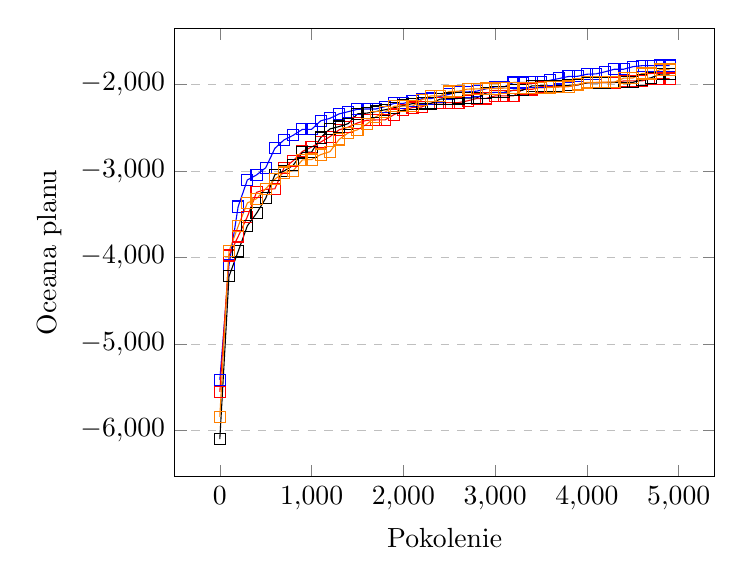
\begin{tikzpicture}
\begin{axis}[
    xlabel={Pokolenie},
    ylabel={Oceana planu},
    ymajorgrids=true,
    grid style=dashed,
]

\addplot[
    color=blue,
    mark=square,
    ]
    coordinates {
(0, -5416.999999999999)(100, -4088.1999999999994)(200, -3408.1999999999994)(300, -3101.1999999999994)(400, -3043.1999999999994)(500, -2960.1999999999994)(600, -2735.2000000000003)(700, -2637.4)(800, -2583.9999999999995)(900, -2515.6)(1000, -2515.6)(1100, -2416.6)(1200, -2388.8)(1300, -2336.8)(1400, -2310.8)(1500, -2283.8)(1600, -2280.2)(1700, -2280.2)(1800, -2253.0)(1900, -2215.0)(2000, -2215.0)(2100, -2191.2)(2200, -2161.8)(2300, -2159.6)(2400, -2134.8)(2500, -2109.8)(2600, -2082.8)(2700, -2082.8)(2800, -2073.8)(2900, -2047.0)(3000, -2024.0)(3100, -2024.0)(3200, -1974.0)(3300, -1974.0)(3400, -1972.0)(3500, -1972.0)(3600, -1948.0)(3700, -1927.0)(3800, -1904.0)(3900, -1902.0)(4000, -1878.2)(4100, -1874.2)(4200, -1849.2)(4300, -1820.2)(4400, -1820.2)(4500, -1791.2000000000003)(4600, -1779.2)(4700, -1779.2)(4800, -1778.2)(4900, -1778.2)
    };
    
    \addplot[
    color=red,
    mark=square,
    ]
    coordinates {
(0, -5553.0)(100, -3974.8)(200, -3754.600000000001)(300, -3526.6000000000004)(400, -3244.2000000000003)(500, -3210.0)(600, -3203.8)(700, -2959.600000000001)(800, -2878.8)(900, -2771.2)(1000, -2720.2000000000003)(1100, -2662.4)(1200, -2600.5999999999995)(1300, -2521.5999999999995)(1400, -2489.6)(1500, -2441.6)(1600, -2410.8)(1700, -2406.8)(1800, -2406.8)(1900, -2344.4)(2000, -2292.4)(2100, -2263.6000000000004)(2200, -2256.6000000000004)(2300, -2212.0)(2400, -2208.8)(2500, -2206.8)(2600, -2206.8)(2700, -2185.8)(2800, -2159.0)(2900, -2158.0)(3000, -2129.0)(3100, -2129.0)(3200, -2129.0)(3300, -2053.8)(3400, -2053.8)(3500, -2022.4)(3600, -2022.4)(3700, -2022.4)(3800, -2021.2)(3900, -2001.4)(4000, -1976.4)(4100, -1974.4)(4200, -1974.4)(4300, -1974.4)(4400, -1955.6000000000001)(4500, -1955.6000000000001)(4600, -1955.6000000000001)(4700, -1928.6000000000001)(4800, -1928.6000000000001)(4900, -1928.6000000000001)
    };
    
        \addplot[
    color=black,
    mark=square,
    ]
    coordinates {
	(0, -6098.999999999999)(100, -4215.799999999999)(200, -3927.7999999999997)(300, -3631.6000000000004)(400, -3487.3999999999996)(500, -3313.4)(600, -3040.6000000000004)(700, -2997.8)(800, -2930.6)(900, -2782.3999999999996)(1000, -2778.3999999999996)(1100, -2610.7999999999997)(1200, -2510.5999999999995)(1300, -2483.5999999999995)(1400, -2449.7999999999997)(1500, -2336.2)(1600, -2328.2)(1700, -2310.0)(1800, -2289.3999999999996)(1900, -2264.3999999999996)(2000, -2239.3999999999996)(2100, -2218.3999999999996)(2200, -2216.3999999999996)(2300, -2216.3999999999996)(2400, -2166.2)(2500, -2159.2)(2600, -2158.2)(2700, -2153.3999999999996)(2800, -2151.3999999999996)(2900, -2095.3999999999996)(3000, -2088.3999999999996)(3100, -2087.2)(3200, -2063.2)(3300, -2063.2)(3400, -2013.3999999999999)(3500, -2010.6)(3600, -2010.6)(3700, -2010.6)(3800, -2006.4)(3900, -2001.1999999999998)(4000, -1978.1999999999998)(4100, -1977.1999999999998)(4200, -1974.8)(4300, -1972.6)(4400, -1972.6)(4500, -1972.6)(4600, -1943.6)(4700, -1918.6)(4800, -1875.6)(4900, -1875.6)
    };
    
            \addplot[
    color=orange,
    mark=square,
    ]
    coordinates {
	(0, -5841.2)(100, -3926.9999999999995)(200, -3636.1999999999994)(300, -3367.6)(400, -3317.6)(500, -3201.6)(600, -3091.7999999999997)(700, -3015.4)(800, -2993.4)(900, -2869.5999999999995)(1000, -2864.5999999999995)(1100, -2807.3999999999996)(1200, -2773.7999999999993)(1300, -2632.399999999999)(1400, -2556.5999999999995)(1500, -2520.7999999999993)(1600, -2456.6000000000004)(1700, -2370.0)(1800, -2316.6000000000004)(1900, -2248.2000000000003)(2000, -2247.2)(2100, -2247.2)(2200, -2173.4000000000005)(2300, -2128.0)(2400, -2128.0)(2500, -2077.8)(2600, -2075.0)(2700, -2050.0)(2800, -2048.0)(2900, -2044.0000000000002)(3000, -2044.0000000000002)(3100, -2039.2000000000003)(3200, -2035.2000000000003)(3300, -2035.2000000000003)(3400, -2035.2000000000003)(3500, -2035.2000000000003)(3600, -2031.0000000000002)(3700, -2025.0000000000002)(3800, -2021.0000000000002)(3900, -1996.0000000000002)(4000, -1973.0000000000002)(4100, -1972.8000000000002)(4200, -1970.8000000000002)(4300, -1968.8)(4400, -1923.8)(4500, -1921.8)(4600, -1869.8)(4700, -1869.8)(4800, -1823.8)(4900, -1823.8)
    };


\end{axis}
\end{tikzpicture}
\caption{Zmiana oceny planu podczas ewolucji badana co 100 pokoleń. \newline
Rozmiar populacji = 10, Liczba pokoleń = 5000, Liczba mutacji = 0.5\% krotek\newline
(więcej=lepiej)}\label{rys:graph_0_5}
\end{figure}

	Ostatni zestaw testów został przeprowadzony po jednym teście z każdego z powyższych zestawów ze zmianą liczby pokoleń na 10000. Takie ustawienie parametrów pozwoliło na znalezienie ciężkich do przejścia progów dla każdego ustawienia. Testy zostały zestawione w ramach jednego wykresu w celu ułatwienia porównania otrzymanych wyników (zob.~rysunek~\ref{rys:graph_all}). Zauważyć można, że dla wartości 3\% oraz 2\% bardzo szybko napotkany zostaje próg nie do przekroczenia przez zbyt dużą losowość. Przez taki próg marnowane są ogromne zasoby obliczeniowe generujące koszty, bez idącego za nimi oczekiwanego wzrostu jakości uzyskanego planu. Z wykresu bardzo szybko wywnioskować można, że najlepszym ustawieniem jest liczba mutacji = 0.5\%. Przez pełen okres wykonywania testu dla tego parametru jakość otrzymywanego planu zwiększała się. Zauważyć można, że optymalnym ustawieniem parametrów dla zaimplementowanego algorytmu jest: rozmiar populacji = 10, liczba pokoleń = 1500, liczba mutacji = 0.5\% liczby krotek w liście (zaokrąglone w dół). Z rysunku przeczytać można, że po przekroczeniu ok.1500 pokolenia dla liczby mutacji = 0.5\% wykres znacznie się spłaszcza co oznacza, że wykorzystując dużą ilość zasobów przez kolejne 8500 pokoleń nie jest otrzymywany już oczekiwany wzrostu jakości.

\begin{figure}[H]
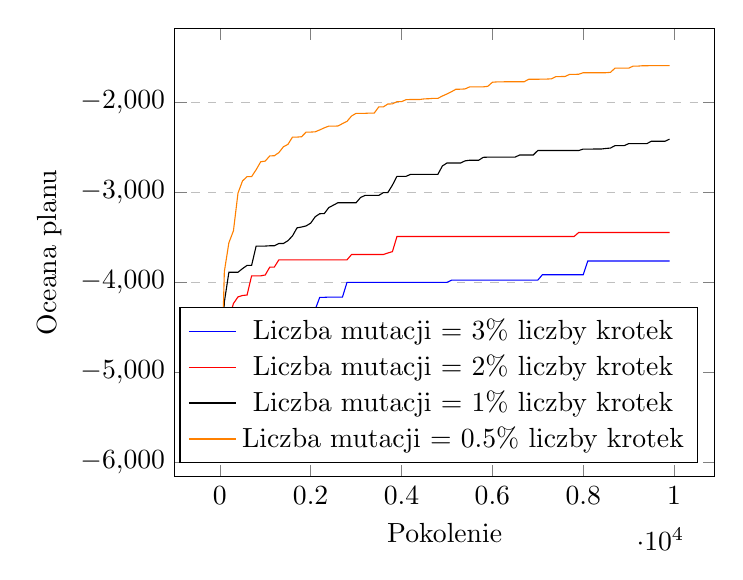
\begin{tikzpicture}
\begin{axis}[
    xlabel={Pokolenie},
    ylabel={Oceana planu},
    ymajorgrids=true,
    grid style=dashed,
    legend pos=south east,
]

\addplot[
    color=blue,
    ]
    coordinates {
	(0, -5694.800000000001)(100, -4786.399999999999)(200, -4730.8)(300, -4730.400000000001)(400, -4701.000000000001)(500, -4524.200000000001)(600, -4524.200000000001)(700, -4354.2)(800, -4354.2)(900, -4354.2)(1000, -4354.2)(1100, -4354.2)(1200, -4354.2)(1300, -4354.2)(1400, -4354.2)(1500, -4354.2)(1600, -4302.000000000001)(1700, -4302.000000000001)(1800, -4302.000000000001)(1900, -4302.000000000001)(2000, -4302.000000000001)(2100, -4302.000000000001)(2200, -4166.4)(2300, -4166.4)(2400, -4163.6)(2500, -4163.6)(2600, -4163.6)(2700, -4163.6)(2800, -3999.9999999999995)(2900, -3999.9999999999995)(3000, -3999.9999999999995)(3100, -3999.9999999999995)(3200, -3999.9999999999995)(3300, -3999.9999999999995)(3400, -3999.9999999999995)(3500, -3999.9999999999995)(3600, -3999.9999999999995)(3700, -3999.9999999999995)(3800, -3999.9999999999995)(3900, -3999.9999999999995)(4000, -3999.9999999999995)(4100, -3999.9999999999995)(4200, -3999.9999999999995)(4300, -3999.9999999999995)(4400, -3999.9999999999995)(4500, -3999.9999999999995)(4600, -3999.9999999999995)(4700, -3999.9999999999995)(4800, -3999.9999999999995)(4900, -3999.9999999999995)(5000, -3999.9999999999995)(5100, -3975.3999999999996)(5200, -3975.3999999999996)(5300, -3975.3999999999996)(5400, -3975.3999999999996)(5500, -3975.3999999999996)(5600, -3975.3999999999996)(5700, -3975.3999999999996)(5800, -3975.3999999999996)(5900, -3975.3999999999996)(6000, -3975.3999999999996)(6100, -3975.3999999999996)(6200, -3975.3999999999996)(6300, -3975.3999999999996)(6400, -3975.3999999999996)(6500, -3975.3999999999996)(6600, -3975.3999999999996)(6700, -3975.3999999999996)(6800, -3975.3999999999996)(6900, -3975.3999999999996)(7000, -3975.3999999999996)(7100, -3915.3999999999996)(7200, -3915.3999999999996)(7300, -3915.3999999999996)(7400, -3915.3999999999996)(7500, -3915.3999999999996)(7600, -3915.3999999999996)(7700, -3915.3999999999996)(7800, -3915.3999999999996)(7900, -3915.3999999999996)(8000, -3915.3999999999996)(8100, -3762.2000000000003)(8200, -3762.2000000000003)(8300, -3762.2000000000003)(8400, -3762.2000000000003)(8500, -3762.2000000000003)(8600, -3762.2000000000003)(8700, -3762.2000000000003)(8800, -3762.2000000000003)(8900, -3762.2000000000003)(9000, -3762.2000000000003)(9100, -3762.2000000000003)(9200, -3762.2000000000003)(9300, -3762.2000000000003)(9400, -3762.2000000000003)(9500, -3762.2000000000003)(9600, -3762.2000000000003)(9700, -3762.2000000000003)(9800, -3762.2000000000003)(9900, -3762.2000000000003)
    };\addlegendentry{Liczba mutacji = 3\% liczby krotek}
    
\addplot[
    color=red,
    ]
    coordinates {
(0, -5366.2)(100, -4468.0)(200, -4408.4)(300, -4235.399999999999)(400, -4161.5999999999985)(500, -4145.999999999998)(600, -4140.5999999999985)(700, -3927.199999999999)(800, -3927.199999999999)(900, -3927.199999999999)(1000, -3917.5999999999995)(1100, -3829.7999999999993)(1200, -3829.7999999999993)(1300, -3748.7999999999993)(1400, -3748.7999999999993)(1500, -3748.7999999999993)(1600, -3748.7999999999993)(1700, -3748.7999999999993)(1800, -3748.7999999999993)(1900, -3748.7999999999993)(2000, -3748.7999999999993)(2100, -3748.7999999999993)(2200, -3748.7999999999993)(2300, -3748.7999999999993)(2400, -3748.7999999999993)(2500, -3748.7999999999993)(2600, -3748.7999999999993)(2700, -3748.7999999999993)(2800, -3748.7999999999993)(2900, -3689.9999999999995)(3000, -3689.9999999999995)(3100, -3689.9999999999995)(3200, -3689.9999999999995)(3300, -3689.9999999999995)(3400, -3689.9999999999995)(3500, -3689.9999999999995)(3600, -3689.9999999999995)(3700, -3672.7999999999993)(3800, -3657.599999999999)(3900, -3489.1999999999994)(4000, -3489.1999999999994)(4100, -3489.1999999999994)(4200, -3489.1999999999994)(4300, -3489.1999999999994)(4400, -3489.1999999999994)(4500, -3489.1999999999994)(4600, -3489.1999999999994)(4700, -3489.1999999999994)(4800, -3489.1999999999994)(4900, -3489.1999999999994)(5000, -3489.1999999999994)(5100, -3489.1999999999994)(5200, -3489.1999999999994)(5300, -3489.1999999999994)(5400, -3489.1999999999994)(5500, -3489.1999999999994)(5600, -3489.1999999999994)(5700, -3489.1999999999994)(5800, -3489.1999999999994)(5900, -3489.1999999999994)(6000, -3489.1999999999994)(6100, -3489.1999999999994)(6200, -3489.1999999999994)(6300, -3489.1999999999994)(6400, -3489.1999999999994)(6500, -3489.1999999999994)(6600, -3489.1999999999994)(6700, -3489.1999999999994)(6800, -3489.1999999999994)(6900, -3489.1999999999994)(7000, -3489.1999999999994)(7100, -3489.1999999999994)(7200, -3489.1999999999994)(7300, -3489.1999999999994)(7400, -3489.1999999999994)(7500, -3489.1999999999994)(7600, -3489.1999999999994)(7700, -3489.1999999999994)(7800, -3489.1999999999994)(7900, -3444.5999999999985)(8000, -3444.5999999999985)(8100, -3444.5999999999985)(8200, -3444.5999999999985)(8300, -3444.5999999999985)(8400, -3444.5999999999985)(8500, -3444.5999999999985)(8600, -3444.5999999999985)(8700, -3444.5999999999985)(8800, -3444.5999999999985)(8900, -3444.5999999999985)(9000, -3444.5999999999985)(9100, -3444.5999999999985)(9200, -3444.5999999999985)(9300, -3444.5999999999985)(9400, -3444.5999999999985)(9500, -3444.5999999999985)(9600, -3444.5999999999985)(9700, -3444.5999999999985)(9800, -3444.5999999999985)(9900, -3444.5999999999985)
    };\addlegendentry{Liczba mutacji = 2\% liczby krotek}
    
\addplot[
    color=black,
    ]
    coordinates {
(0, -5319.400000000001)(100, -4218.4)(200, -3886.9999999999995)(300, -3886.9999999999995)(400, -3886.9999999999995)(500, -3846.399999999999)(600, -3810.999999999999)(700, -3810.999999999999)(800, -3595.6)(900, -3595.6)(1000, -3595.6)(1100, -3592.4)(1200, -3592.4)(1300, -3567.4)(1400, -3567.4)(1500, -3535.7999999999997)(1600, -3482.6)(1700, -3392.8)(1800, -3383.7999999999997)(1900, -3371.4)(2000, -3340.8000000000006)(2100, -3269.600000000001)(2200, -3236.000000000001)(2300, -3233.600000000001)(2400, -3167.2000000000003)(2500, -3140.4)(2600, -3113.4)(2700, -3113.4)(2800, -3113.4)(2900, -3113.4)(3000, -3113.4)(3100, -3054.2000000000003)(3200, -3031.7999999999997)(3300, -3031.7999999999997)(3400, -3031.7999999999997)(3500, -3031.7999999999997)(3600, -3001.0000000000005)(3700, -2999.8)(3800, -2917.4)(3900, -2819.600000000001)(4000, -2819.600000000001)(4100, -2819.600000000001)(4200, -2797.600000000001)(4300, -2797.600000000001)(4400, -2797.600000000001)(4500, -2797.600000000001)(4600, -2797.600000000001)(4700, -2797.600000000001)(4800, -2797.600000000001)(4900, -2704.2000000000007)(5000, -2671.2000000000007)(5100, -2671.2000000000007)(5200, -2671.2000000000007)(5300, -2671.2000000000007)(5400, -2647.2000000000007)(5500, -2640.2000000000003)(5600, -2640.2000000000003)(5700, -2640.2000000000003)(5800, -2608.0000000000005)(5900, -2606.0000000000005)(6000, -2606.0000000000005)(6100, -2606.0000000000005)(6200, -2606.0000000000005)(6300, -2606.0000000000005)(6400, -2606.0000000000005)(6500, -2606.0000000000005)(6600, -2582.0000000000005)(6700, -2582.0000000000005)(6800, -2582.0000000000005)(6900, -2582.0000000000005)(7000, -2532.2)(7100, -2532.2)(7200, -2532.2)(7300, -2532.2)(7400, -2532.2)(7500, -2532.2)(7600, -2532.2)(7700, -2532.2)(7800, -2532.2)(7900, -2532.2)(8000, -2516.0)(8100, -2516.0)(8200, -2516.0)(8300, -2515.2)(8400, -2515.2)(8500, -2509.4)(8600, -2504.6000000000004)(8700, -2478.4)(8800, -2478.4)(8900, -2478.4)(9000, -2455.6000000000004)(9100, -2455.6000000000004)(9200, -2455.6000000000004)(9300, -2455.6000000000004)(9400, -2455.6000000000004)(9500, -2429.2)(9600, -2429.2)(9700, -2429.2)(9800, -2429.2)(9900, -2405.8)
    };\addlegendentry{Liczba mutacji = 1\% liczby krotek}
    
    \addplot[
    color=orange,
    ]
    coordinates {
(0, -5745.199999999999)(100, -3879.0)(200, -3558.4000000000005)(300, -3426.4)(400, -3006.7999999999997)(500, -2870.6)(600, -2822.6)(700, -2822.6)(800, -2746.2000000000003)(900, -2657.8)(1000, -2649.8)(1100, -2592.2000000000003)(1200, -2590.2000000000003)(1300, -2555.6000000000004)(1400, -2490.6000000000004)(1500, -2463.6000000000004)(1600, -2382.8)(1700, -2382.8)(1800, -2378.8)(1900, -2327.0)(2000, -2327.0)(2100, -2323.8)(2200, -2302.8)(2300, -2279.8)(2400, -2260.4)(2500, -2260.4)(2600, -2259.6000000000004)(2700, -2232.8)(2800, -2207.8)(2900, -2148.2)(3000, -2118.2)(3100, -2118.2)(3200, -2118.2)(3300, -2115.4)(3400, -2115.4)(3500, -2046.4000000000003)(3600, -2046.4000000000003)(3700, -2014.4)(3800, -2013.4)(3900, -1988.4)(4000, -1988.4)(4100, -1966.4)(4200, -1964.4)(4300, -1964.4)(4400, -1964.4)(4500, -1957.4)(4600, -1955.6000000000001)(4700, -1951.6000000000001)(4800, -1951.6000000000001)(4900, -1925.6000000000001)(5000, -1902.6000000000001)(5100, -1877.6)(5200, -1849.8)(5300, -1849.6000000000001)(5400, -1846.6000000000001)(5500, -1823.6000000000001)(5600, -1823.6000000000001)(5700, -1823.6000000000001)(5800, -1823.6000000000001)(5900, -1817.6000000000001)(6000, -1772.4)(6100, -1768.4)(6200, -1768.4)(6300, -1766.4)(6400, -1766.4)(6500, -1766.4)(6600, -1766.4)(6700, -1766.4)(6800, -1739.4)(6900, -1739.4)(7000, -1739.0)(7100, -1737.0)(7200, -1737.0)(7300, -1734.0)(7400, -1709.0)(7500, -1709.0)(7600, -1708.0)(7700, -1685.0)(7800, -1685.0)(7900, -1683.0)(8000, -1666.0)(8100, -1666.0)(8200, -1666.0)(8300, -1666.0)(8400, -1666.0)(8500, -1666.0)(8600, -1662.0)(8700, -1615.8)(8800, -1615.8)(8900, -1615.8)(9000, -1615.8)(9100, -1592.8)(9200, -1592.8)(9300, -1588.8)(9400, -1588.8)(9500, -1586.8)(9600, -1586.8)(9700, -1586.8)(9800, -1586.8)(9900, -1586.8)
    };\addlegendentry{Liczba mutacji = 0.5\% liczby krotek}
    


\end{axis}
\end{tikzpicture}
\caption{Zmiana oceny planu podczas ewolucji badana co 100 pokoleń. \newline
Rozmiar populacji = 10, Liczba pokoleń = 5000\newline
(więcej=lepiej)}\label{rys:graph_all}
\end{figure}
	
	 

